\documentclass[11pt,a4paper]{article}
\usepackage[margin=2.2cm]{geometry}
\usepackage{booktabs}
\usepackage{graphicx}
\usepackage{amsmath}
\usepackage{float}
\usepackage[hidelinks]{hyperref}

\title{Assignment 4: Embeddings and Mixture of Experts}
\author{}
\date{}

\begin{document}
\maketitle
\vspace{-1.5cm}

\section{Part A: Learning Image Embeddings from Scratch}

We trained two embedding models on Fashion-MNIST (60k training, 10k test, 10 classes) using small convolutional architectures with 16-dimensional latent spaces.

\textbf{A1 -- Autoencoder.} The autoencoder uses a Conv-Conv-Linear encoder mapping $28\times28$ images to 16-d vectors, and a symmetric decoder reconstructing the input. After 10 epochs with MSE loss, reconstruction loss decreased from 0.054 to 0.014. Reconstructions preserve overall shape and structure but lose fine details such as text on shirts and sharp edges, which is expected from a 16-d bottleneck.

\textbf{A2 -- Contrastive (Siamese).} The Siamese network uses the same encoder backbone trained with contrastive loss: positive pairs (same class) are pulled together, negative pairs (different class) are pushed apart with margin 1.0. Contrastive loss decreased from 0.108 to 0.075 over 10 epochs.

\begin{figure}[H]
\centering
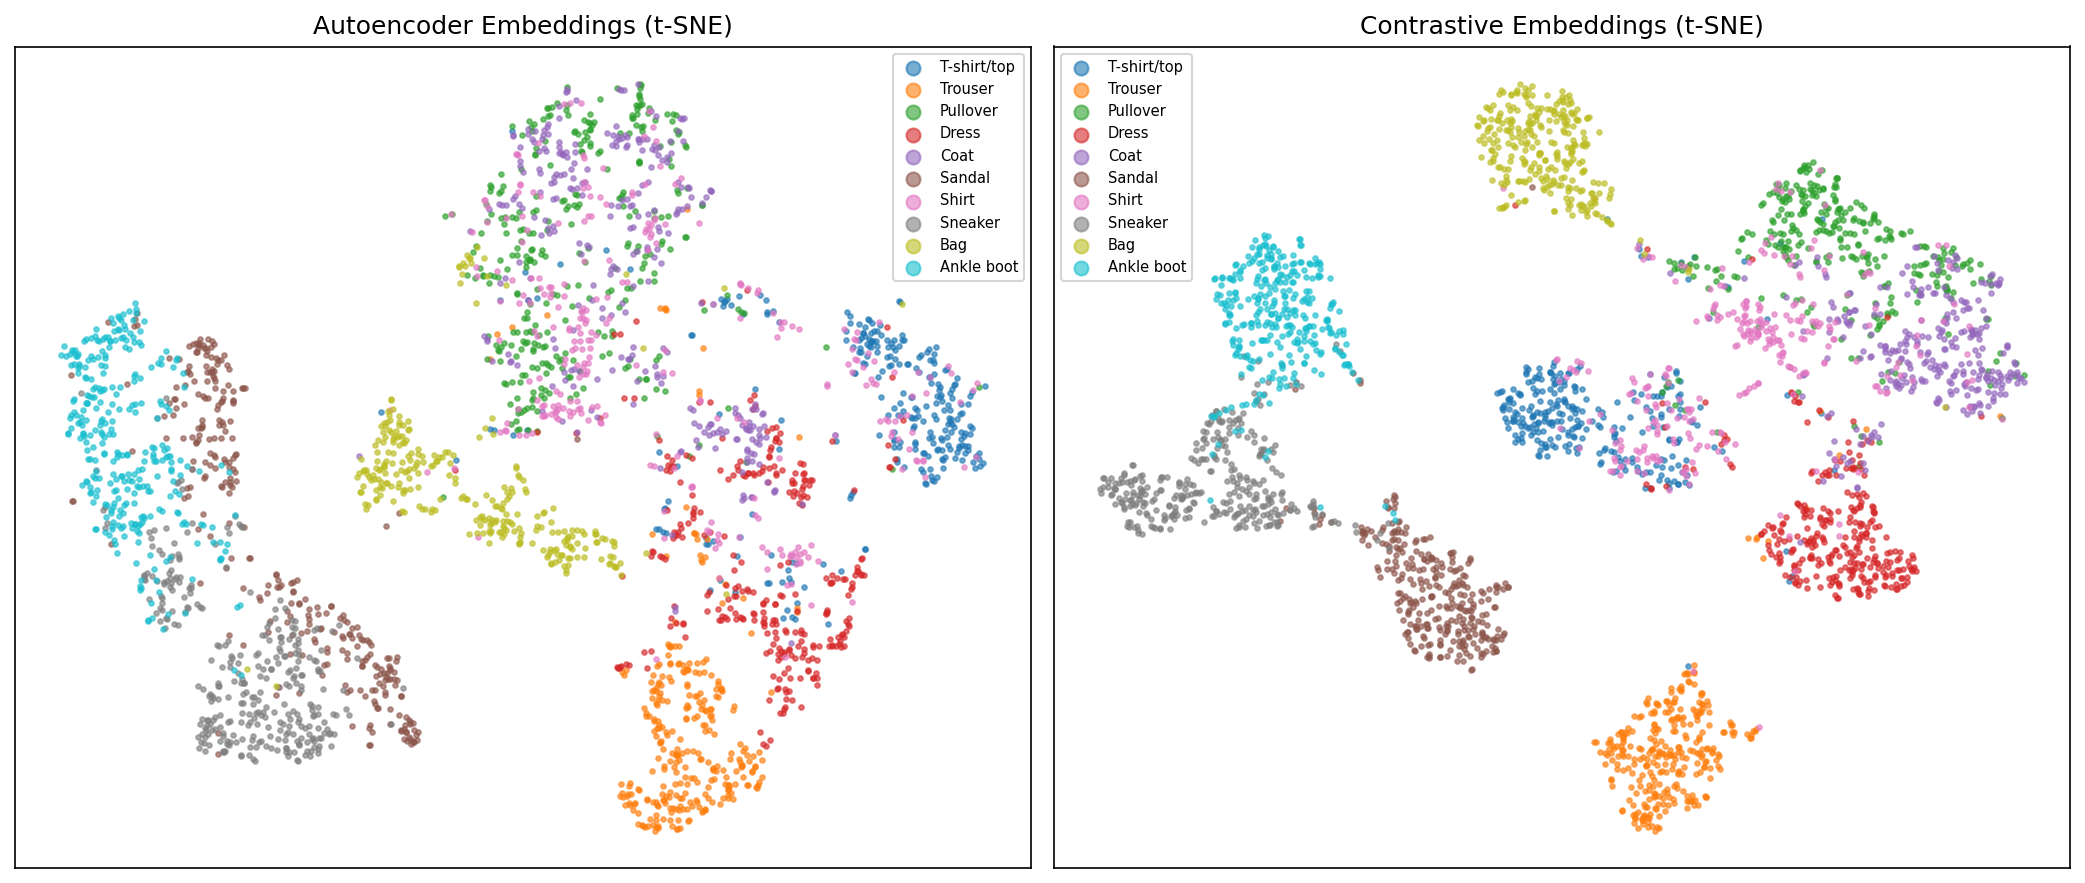
\includegraphics[width=0.95\textwidth]{part_a_embeddings_tsne.png}
\caption{t-SNE of autoencoder (left) and contrastive (right) embeddings on Fashion-MNIST test set.}
\end{figure}

The t-SNE visualisations show that both methods produce meaningful clusters. The autoencoder embeddings form loose, overlapping groups since the reconstruction objective does not explicitly encourage class separation. The contrastive embeddings produce tighter, better-separated clusters because the loss directly optimises for inter-class distance. Both methods confuse visually similar classes (T-shirt/Shirt, Sneaker/Ankle boot), which is expected given the pixel-level similarity.

\section{Part B: Foundation Model Embeddings (CLIP)}

We extracted 512-d embeddings from CLIP ViT-B/32 on the same Fashion-MNIST test set and compared all three methods using $k$-NN ($k{=}5$) classification accuracy as an embedding quality metric.

\begin{table}[H]
\centering
\begin{tabular}{lccc}
\toprule
Method & Dim & kNN Acc \\
\midrule
Autoencoder & 16 & 0.804 \\
Contrastive & 16 & \textbf{0.861} \\
CLIP ViT-B/32 & 512 & 0.851 \\
\bottomrule
\end{tabular}
\caption{Embedding quality measured by $k$-NN classification accuracy.}
\end{table}

The contrastive embeddings slightly outperformed CLIP (86.1\% vs 85.1\%) despite being 32$\times$ lower dimensional. This is because the contrastive model was trained directly on Fashion-MNIST, learning domain-specific features, whereas CLIP was trained on natural images and text and has never seen grayscale clothing sketches. CLIP's embeddings still perform well because its large-scale pretraining captures general visual concepts that transfer across domains. The autoencoder embeddings are weakest (80.4\%) because reconstruction does not require class-discriminative features -- two visually different shirts may map to distant points while a shirt and a coat with similar silhouettes map nearby.

\begin{figure}[H]
\centering
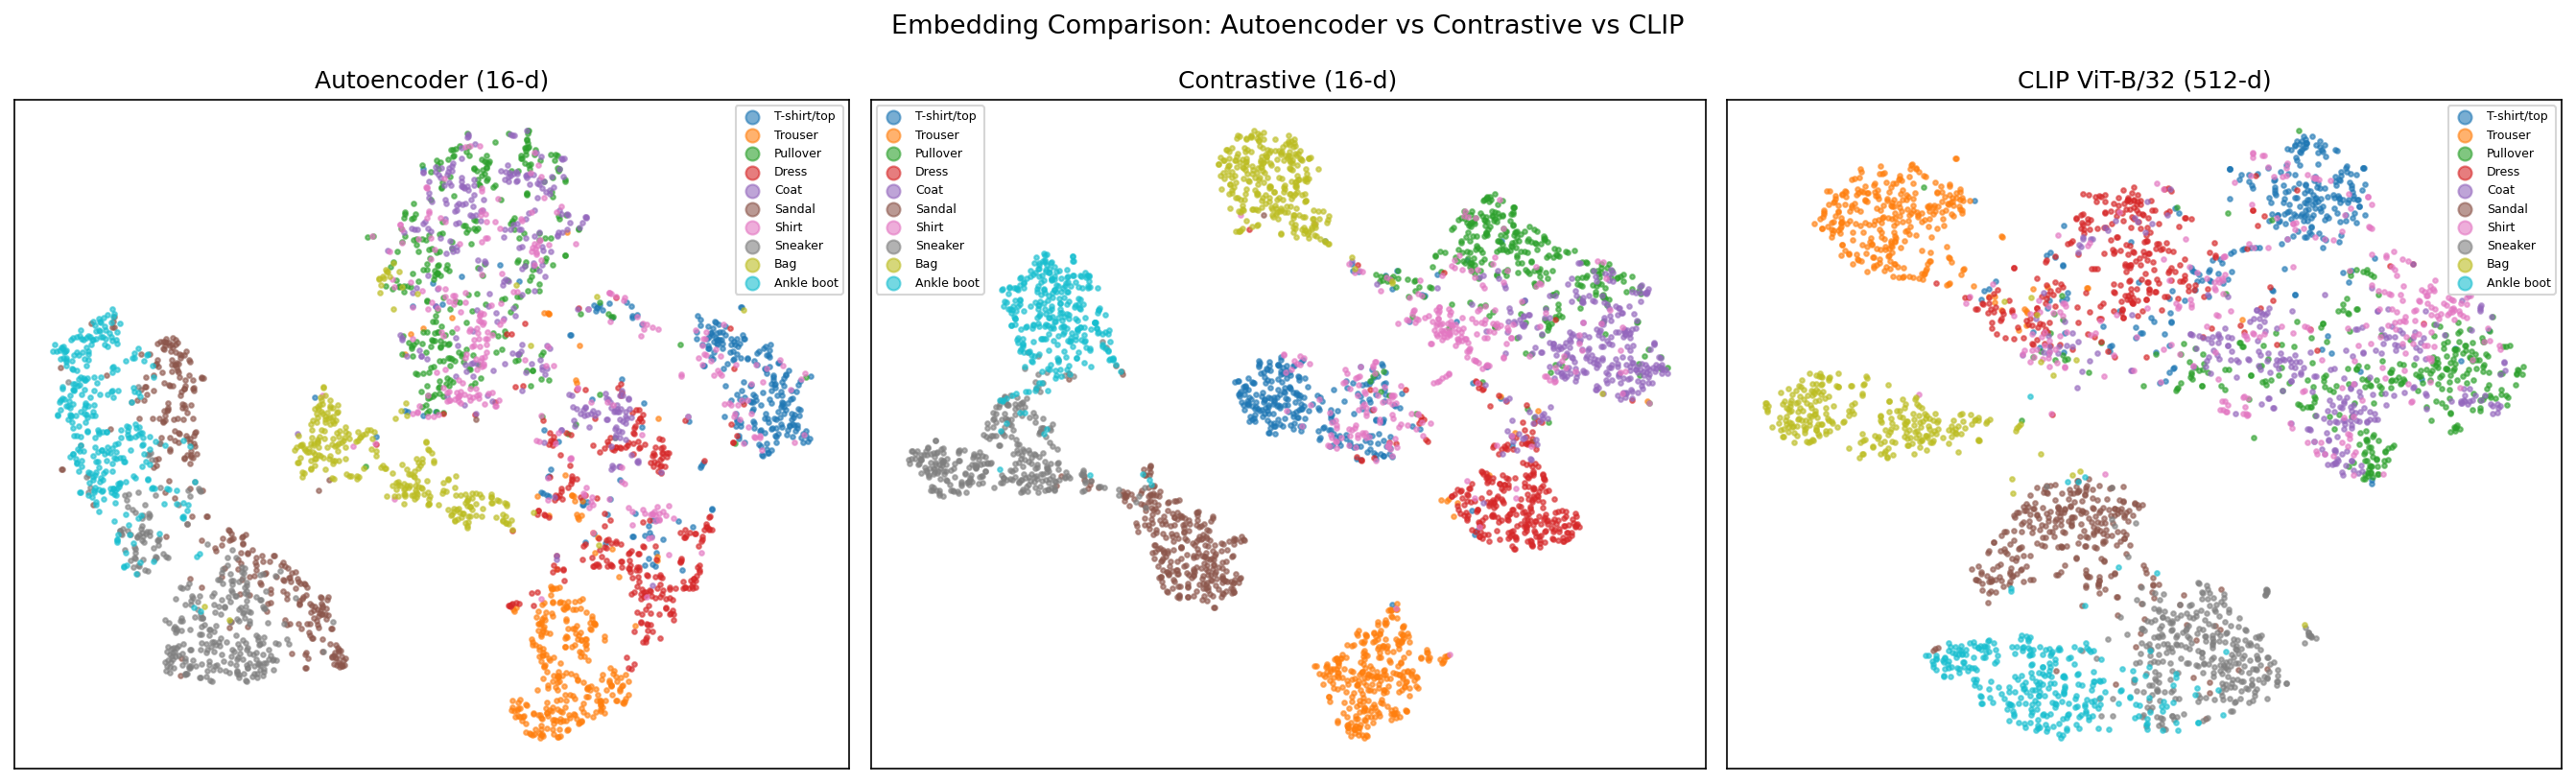
\includegraphics[width=0.99\textwidth]{part_b_embedding_comparison.png}
\caption{t-SNE comparison: Autoencoder vs Contrastive vs CLIP embeddings.}
\end{figure}

The CLIP t-SNE plot shows well-defined clusters but with more inter-class mixing than the contrastive model, confirming the quantitative kNN results. CLIP separates semantically distinct categories (Bag, Trouser, Sandal) cleanly, but struggles with the fine-grained clothing distinctions that the task-specific contrastive model learned.

\section{Part C: Mixture of Experts}

We built a Mixture of Experts (MoE) system using four frozen expert classifiers from Assignment~3 (trained on CIFAR-10 for 20 epochs each) and a lightweight CNN-based gating network. The router takes an image as input and produces softmax weights $g_i(x)$ over the experts. The final prediction is $z(x) = \sum_{i=1}^{K} g_i(x)\, z_i(x)$, where $z_i(x)$ is expert $i$'s logit vector.

\begin{table}[H]
\centering
\begin{tabular}{lc}
\toprule
Model & Test Acc \\
\midrule
ResNet (expert) & 0.885 \\
Inception (expert) & 0.852 \\
SqueezeNet (expert) & 0.753 \\
SuperNet (expert) & 0.868 \\
\midrule
MoE (router) & \textbf{0.893} \\
\bottomrule
\end{tabular}
\caption{Individual expert and MoE test accuracy on CIFAR-10.}
\end{table}

The MoE achieved 89.3\%, surpassing the best individual expert (ResNet at 88.5\%) by 0.9 percentage points. The router learned to assign approximately 71\% weight to ResNet and 27\% to SuperNet across all classes, effectively ignoring SqueezeNet (0\%) and Inception (1.5\%). This weighting is consistent with individual expert performance and shows the router successfully identified which experts are most reliable. The gating weights were remarkably uniform across classes, suggesting that on CIFAR-10 the expert strengths are not class-specific but rather reflect overall model quality.

\begin{figure}[H]
\centering
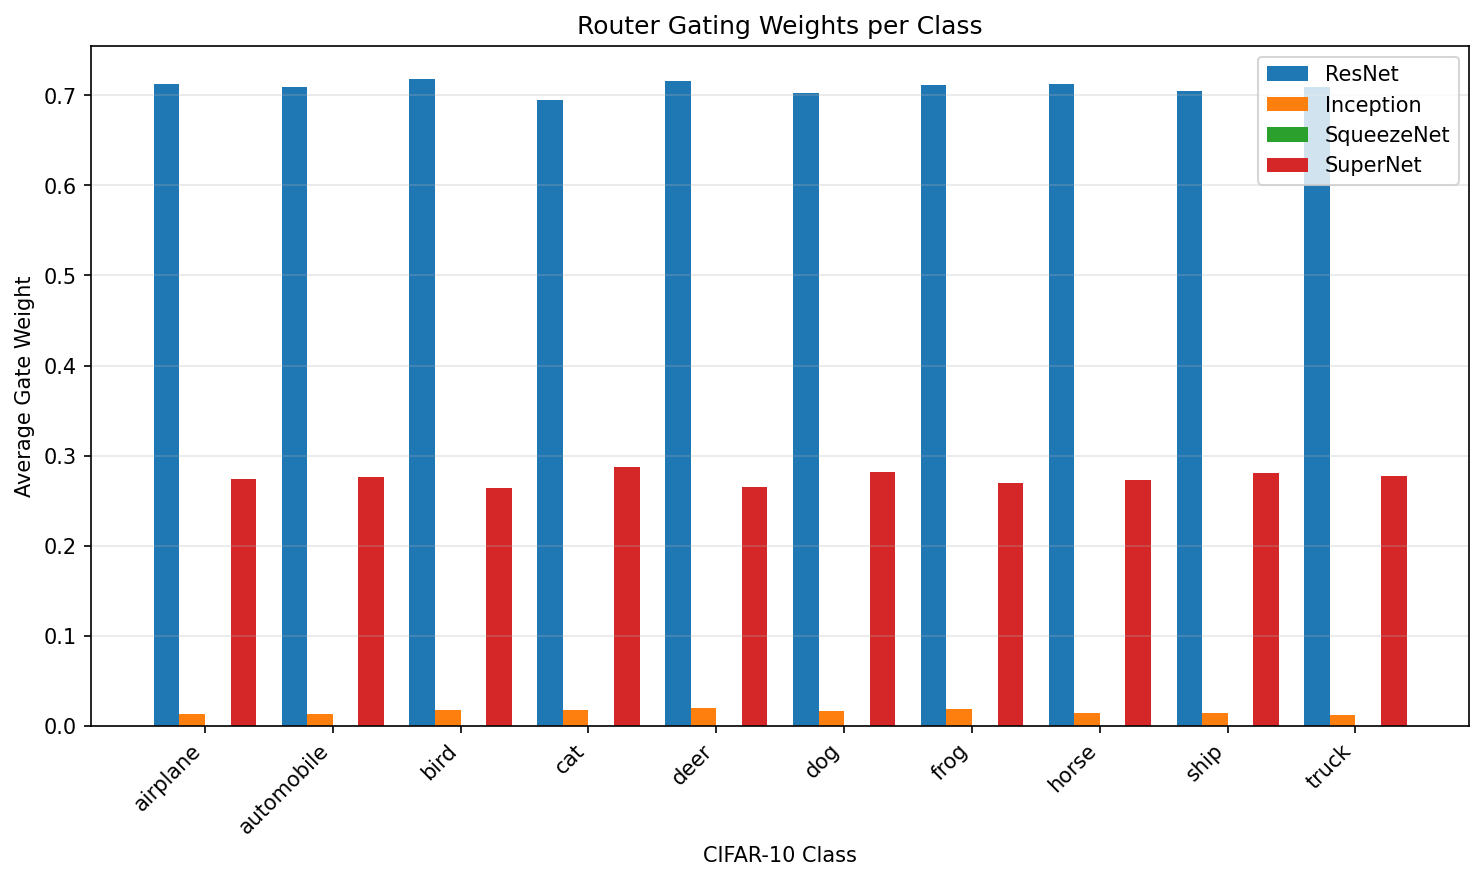
\includegraphics[width=0.7\textwidth]{part_c_gating_weights.png}
\caption{Average router gating weights per CIFAR-10 class.}
\end{figure}

The near-uniform gating pattern suggests that a more diverse set of experts (e.g., models with complementary strengths on different classes) would allow the router to learn more interesting specialisation patterns and potentially achieve larger accuracy gains over the best individual expert.

\end{document}
